\documentclass[oneside]{book}

% 注意宏包顺序,有可能会报错
\usepackage{ctex}% 中文支持
\usepackage{geometry}% 用于页面设置
\usepackage[dvipsnames, svgnames, x11names]{xcolor}% 颜色支持
\usepackage{graphics}% 图形支持
\usepackage[
colorlinks=true,
linkcolor=Navy,
urlcolor=Navy,
citecolor=Navy,
anchorcolor=Navy
]{hyperref}% 设置超链接颜色
\usepackage{enumerate}% 枚举支持
\usepackage{tcolorbox}% 支持更好的文本框
\usepackage[english]{babel}% 载入美式英语断字模板
\usepackage{ulem}% 用于支持在字体上做下划线、波浪线等记号

% 设置为A4纸,边距适中模式(参考永中office)
\geometry{
	paperwidth = 9cm,
	paperheight = 12.2cm,
	margin = 0cm,
	left = 0.2cm,
	right = 0.2cm,
	top = 0.2cm,
	bottom = 0.5cm
}

\hyphenpenalty = 1000% 断字设置,值越大,断字越少。
\setmainfont{Ubuntu Mono}% 设置全局英文字体
\setlength{\parindent}{2em}% 缩进
\setlength{\parskip}{1ex} % 段间距

\let\svthefootnote\thefootnote

% 把目录区中英文的“Contents”改为中文的“目录”。
\addto\captionsenglish{
	\renewcommand{\contentsname}{目录}
}

% 把章节名称part、chapter换成中文
\usepackage{titlesec}% 可使用\usepackage[center]{titlesec}设置对齐方式
\titleformat{\part}{\centering\Huge\bfseries}{第\,\thepart\,部分}{0em}{\\}
\titleformat{\chapter}{\raggedright\Huge\bfseries}{第\,\thechapter\,章}{1em}{}
%\titleformat{\section}{\raggedright\Large\bfseries}{\,\thesection\,}{1em}{}

\includeonly{
	part1,
}

% 定义指定字体名称与大小的文字输出命令
% 第1个参数:字体名称
% 第2个参数:字体大小
% 第3个参数:文本内容
\newcommand{\SetFont}[3]{
	\setCJKfamilyfont{font1}{#1} \CJKfamily{font1}\fontsize{#2}{#2}{\selectfont #3}
}

% 因为书中大量使用下划线,所以这里定义更为简便的命令来实现
\newcommand{\UL}[1][]{\underline{#1}}


% ------------------ 开始 -------------------

\begin{document}
	
	% ------------------ 封面 -------------------
	\begin{titlepage}
		\pagecolor{black}
		\begin{center}
			\quad\\[20mm]
			\SetFont{FZKai-Z03S}{40}{\textcolor{Gold}{圣\quad 经}}
		\end{center}
	\end{titlepage}
	
	% ------------------ 前言 -------------------
	\frontmatter% 关闭章节序号,页码使用罗马数字
	\restoregeometry% 恢复导言区指定的页面布局。
	\nopagecolor% 清除封面创建时设置的背景色
	
	\pagecolor{WhiteSmoke}
	\begin{center}
		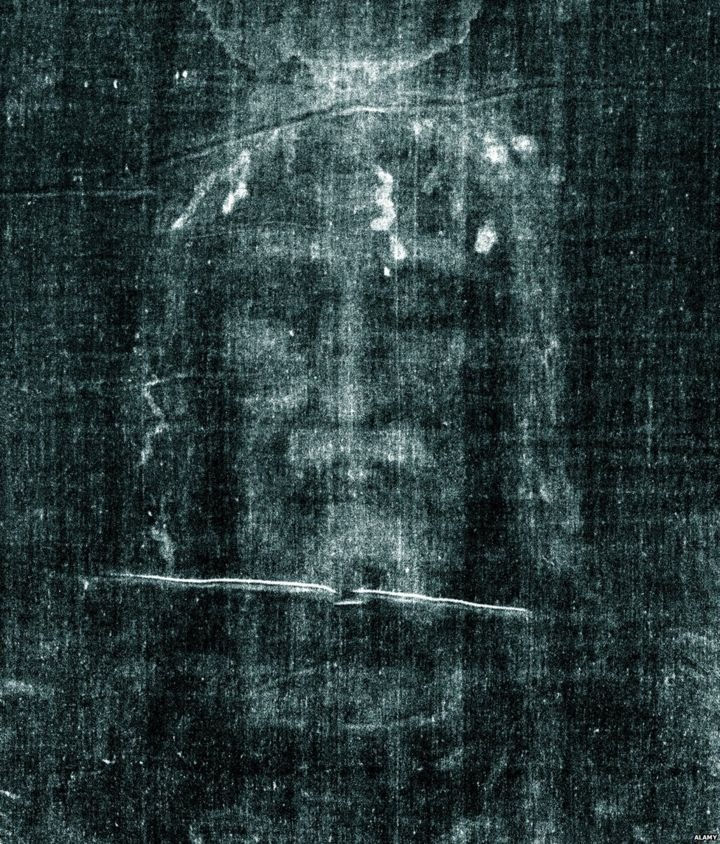
\includegraphics[width=8.5cm]{images/基督的面上闪耀着天主的光荣.png}
		
		\SetFont{zcoolqingkehuangyouti}{11}{“基督的面上闪耀着天主的光荣”}\normalsize\heiti(格后4:6)\songti
	\end{center}
	
	\newpage\normalsize
	\begin{center}
		\quad\\[10mm]
		承蒙联合圣经公会(United Bible Societies)
		
		为这一版本圣经的出版捐赠纸张,指定在中国
		
		大陆发行,谨此致谢!
		
		请为捐赠者祈祷。\\[10mm]
		
		With grateful thanks to United Bible
		
		Societies for the paper donated in
		
		the production of this Bible.
		
		This Bible is designated for distribution within mainland China only.
		
		Please pray for the donors.
	\end{center}
	
	\newpage
	\begin{center}
		\quad\\[15mm]
		\SetFont{FZKai-Z03S}{40}{圣\quad 经}
		\vfill
		\large\heiti 中国天主教主教团 准\normalfont\normalsize
	\end{center}
	
	\newpage
	\quad\\
	版权所有\copyright 思高圣经学会
	\vfill
	\begin{center}
		\Large 圣 经\normalsize
		
		——————————————
		
		发行者:中国天主教主教团
		
		承印者:南京爱德印刷有限公司
		
		准印证号:Z(2018)00000522
	\end{center}
	
	\newpage
	\quad\\\\
	\centerline{\heiti\large 前\qquad 言}\songti\normalsize
	
	\quad
	
	为了满足广大神长教友的需求,经中国天主教主教团批准,现将旧、新约合订本《圣经》印制发行。并再次感谢香港思高圣经学会的帮助。
	
	《圣经》是一部在天主圣神默示下写成的圣书,天主的话是圣教会及众信友的生命泉源,是不可缺少的精神食粮,愿神长教友在圣教会的训导下,虔诚地、认真地阅读、默想《圣经》,聆听基督的圣训,在爱主爱人的道路上不断圣化自己,为主作证。\\\\
	\mbox{\quad}\hfill 中国天主教主教团\mbox{\qquad\quad}\\
	\mbox{\quad}\hfill 2009年2月\mbox{\qquad\qquad}
	
	\newpage
	\quad\\\\
	\centerline{\heiti\large 序}\songti\normalsize
	
	\quad
	
	中文《新旧约》合订本,几经艰辛,终于出版面世了。现在谨以孝爱的心肠,与兴奋的心情,将此书献给我国的天主教会。我们由衷地感谢万善万美之源在天之父,虔恭地恳求他,降福我们的每一位神形恩友。我们明知,如果没有他们精神方面的支持与物质方面的援助,这部\UL[中]译圣经合订本、很难于今日完成。我们更恳求天父,以圣神的恩泽,充溢每位读者的心灵,为光荣他,和他的圣子,我们的救主\UL[耶稣]\UL[基督]。最后,我们以至诚的心,深望每位读者,效法天主之母,童贞圣母\UL[玛利亚],常将天主子\UL[耶稣]\UL[基督]的奥迹,默存于心,反复思念(\uwave{路}2:19、51)。
	
	我们坦诚地说过应说的话以后,兹将有关出版这部合订本的原则与方法,向诸位读者报告如下:
	
	本学会同仁,对本学会以前的译文,作了一次彻底的修订;特别对于《旧约》部分,觉得有重新翻译的必要。这次的修订,一如以往翻译一样,仍旧依据原文,即\UL[希伯来]、\UL[阿剌美]和\UL[希腊]文,间或有时依据古译本,将艰涩的经文稍加修改,很少采用近代学者的臆测。为了促进合一运动,我们在《新约》的修订工作上,曾参考了最近基督教五个圣经公会联合印行的《圣经》希腊版本。这版本是1966年由\UL[艾朗德](Aland)\UL[白赖克](Black)\UL[墨则格](Metzger)\UL[魏革伦](Wikgren)四位极负盛名的学者所细心校勘的。不过,在选择异文方面,有时我们未能尽表赞同或采纳。然而,众所周知,在校勘方面,要想使所有学者的意见,完全趋于一致,几乎是不可能的事;同时,艰深疑难的问题,也实在可说是无法解决;但为了遵守有助于合一运动的措施,我们仍尊重而参考了他们的意见。
	
	在翻译《多俾亚传》和《友弟德传》时,我们采用了《西乃抄卷》,因而与\UL[拉丁]通行本和其他控译本,略有出入,因为这些译本,大半是根据《亚历山大抄卷》或《梵蒂冈抄卷》而译成的。
	
	《德训篇》一书,我们虽译自\UL[希腊]文,但同时也参考了最近在古\UL[开罗]的旧书库中,以及在\UL[死海]近旁的\UL[古木兰],和1965年在\UL[玛撒达]所发现的本书\UL[希伯来]文残卷。为了更进一步了解本书\UL[希腊]译者的愿意,我们自始至终,将\UL[希腊]本,与古\UL[拉丁]译本和《叙利亚培西托》译本,加以比较和对正。至于\UL[拉丁]通行本所特有的辞句,我们仍旧全部保留,以小字体排印;我们如此作,是因为这些经文往往与\UL[希伯来]文残卷和\UL[叙利亚]译本相吻合;尤其因为在\UL[拉丁]教会内,许多世纪以来,在礼仪上采用了这些经文。至于本书的音节,全依\UL[拉丁]通行本排列。
	
	至论《圣咏集》的翻译,虽也译自\UL[希伯来]原文,但我们却作了一个新的尝试,就是放弃了过去无韵文的翻译,而试作有韵文的翻译。采取这种翻译的理由,是为了在礼仪上便于诵读。
	
	为了切合实际,我们尽量缩短了每卷的引言和注释。对于那些欲求圣经高深知识的读者,我们仍建议,请他们参考本学会以前出版的《圣经》各卷注释。对于那些工作繁重与事务缠身,而没有充分时间的读者,我们认为本书的引言、注释以及各种附录和图表,已够他们了解《圣经》的主旨。如果读者能进一步,如圣教会所期望的,以祈祷和默祷的方式阅读本书,则更受益匪浅。
	
	现在再向读者特别介绍本书后面的三种附录,这类附录在\UL[中]文《圣经》方面尚属少见。
	
	一、“历代大司祭一览表”:读者可从这表内,正确地明晰一切有关宗教事务的事实,发生于何时何代,发生在哪一位大司祭的任期中。
	
	二、“圣经与世界大事年表”:在这表内,我们以编年体,将选民的历史,以及与选民有关的其他民族的历史,和我们\UL[中华]民族的历史,加以比较,列表阐明。我们认为这一附录,可使我国同胞,更方便而有效地传诵救恩史。
	
	三、“圣经教义索引”:这是为了符合\UL[梵蒂冈]第二届大公会议的期望,而特别编制的,目的是使信友迅速而无误地,直接从圣经中吸取天主启示的各端要理,走上愈显天父的光荣,生活于基督内的康庄大道。我们希望藉此索引,得到抛砖引玉的效果,就是说,希望每位读者藉此索引,能将救恩史的大纲,加以质的扩充和量的增补。
	
	至于地理图表,以及其他有关圣经的插图,都是参照专家和学者们最新的探讨与研究的心得,而予以重新编制的。本书的题字“圣经”、“旧约”、“新约”、六字,是临自《大秦景教流行中国碑》。
	
	最后,我们愿用一首庄严而又古雅的赞颂辞,向我全国教胞表达我们的心愿,并结束这篇序文:愿光荣藉着天主圣子,在天主圣神内,并在圣教会内,永远归于天主圣父!\\
	
	\mbox{\quad}\hfill 思高圣经学会谨识于香港\\
	\mbox{\quad}\hfill 1968年8月15日\mbox{\quad}\\
	\mbox{\quad}\hfill 圣母升天瞻礼\mbox{\qquad}
	
	\newpage
	\quad
	
	\centerline{\large\textbf{凡\qquad 例}}\normalsize
	
	(一)本书中人名地名,除教会与普通常用者外,大抵依原文音译。
	
	(二)本书引言、注释引用的经文,概以本书译文为根据。
	
	(三)凡后人所加,或由他处窜入的经文,概置于方括弧内。
	
	(四)*号表示原文无,只见于\UL[拉丁]通行本。
	
	(五)《新约》经文引用《旧约》经文,概括以‘ ’引号。
	
	(六)引言、注释内,如引用原书经文,则不标书名,只标章节。
	
	(七)引言、注释内,注明出处时,章数、节数按如下表示:如\uwave{依}3:6,即《依撒意亚》第3章第6节;如一书没有章数,则节数按以下标出:如\uwave{北}8,即《亚北底亚》8节。
	
	% ------------------ 目录 -------------------
	\tableofcontents% 生成目录
	
	% ------------------ 正文 -------------------
	\mainmatter%
	
	\part{旧约}


\chapter*{新旧约全书总论}
《新旧约全书》是数十卷经书的总集。这些经书的特点,在于它们的写成有超乎自然之处,因为这些经书都是在天主对神默感下写成。赐予天主的子民——教会——的礼品。

圣教会自古以来,一致主张这部总集包括《旧约》46卷,《新约》27卷,共计73卷。但大多数的\UL[基督教]派,由于只相信以\UL[希伯来]文写成的书才为圣经,因此现今只有\UL[希腊]原文的《巴路克》、《多俾亚传》、《友弟德传》、《玛加伯》上下、《智慧篇》和《德训篇》7卷,未著录在他们的圣经书目内。而天主教会自古即以\UL[希腊]文七十贤士本为圣经,因而对上述7卷也一律认为是圣经。

这些经书称为“约“,因为其中心思想,是天主与人类所立的盟约。天主与\UL[以色列]民族在\UL[西乃]山上所立的盟约,称为“旧约“;\UL[耶稣]以自己的圣血和圣死为全人类所立的永远盟约,称为“新约“。这些经书又称为“圣经“,是为表示这些书所具有的独特地位和神圣权威。书中所记述的一切,是吾人信仰及道德的大经,又为吾人立身经世的大道。

《旧约》经书的原文,除几卷和几小段外,大都以\UL[希伯来]文写成。后来侨居\UL[北非]受了\UL[希腊]文件影响的\UL[犹太]人,因多不谙\UL[希伯来]文,\UL[犹太]人遂在公元前三至二世纪,将《旧约》各书译为\UL[希腊]文,即今所称的“七十贤士译本“。以后\UL[希腊]文\footnote[0]{原书为“语文“}也成了\UL[罗马]帝国的通用语言,宗徒们在各宣讲福音,为了方便起见,即时常利用这部\UL[希腊]文圣经。为此这部\UL[希腊]文圣经(包括46卷)自初即为教会所尊重,并具有极大的权威。

《新约》各书,全部是以\UL[希腊]文写成,只有《玛窦福音》,原文虽为\UL[阿辣美]文,但很早即已失传;今所留传的,只有\UL[希腊]文本。

《旧约全书》的写成,凡经一千余年(约由公元前1300至100年),而逐渐汇为一集。《新约全书》是公元初世纪宗徒时代的作品。

《新旧约全书》,通常分为三大类:即历史书、先知书和智慧书(或训诲书),这是很广泛的分类。至于作者,《旧约》大多出于先知及其他贤哲的手笔,《新约》是宗徒和宗徒弟子的写作。但因全部圣经都是“因天主的默感写成的“(\uwave[弟]后3:16),经内的话是“由天主所派遣的圣人,在圣神推动之下说出来的“(\uwave[伯]后),为此我们不得不承认圣经的首要作者是天主。所谓“默感“,即是说:圣经的作者与编者(人),在天主的灵性感动之下,写下天主愿向他的子民(旧约与新约的教会)所要说的话,记下天主要他们记述的史事。有时天主也曾向他们透露某些重要的事迹,或直接向他们说话;这样,作者不仅获得了“默感“,同时也获得了“启示“。既然天主是圣经的首要作者,那么圣经上所记载的即是天主的话,即是天主的“圣言“。既然是天主的话,那么圣经上所载的一切,句句都是“真实无误“。就是说:圣经作者在天主默感下所愿表示出来的意义,是不会错误的。但为了解作者所要表达的本意,必须先注意经书中每部书的文体和体裁:是散文或是诗体?是历史或是传奇?是寓言或是训诲?因为每种文体有其独特的意义。同时还应注意作者或编者的时代背景,因为时代不同论事的观点也各有异。比如古代民族,尤其\UL[以色列]人对历史的观点,和今日的史学家的观点,有绝大的不同。尤其圣经的作者或编者,是本着宗教观点来编述历史的过程。他们看历史时,常着眼于天主为历史的推动者和支配者;人民的盛衰兴亡,常系之于他们是否遵守天主的法律。

另一个极重要的问题,是圣经与科学。圣经的作者决无意又教授自然科学(如宇宙学、天文学、生物学、人类学等)为写作的目的。圣经作者的目的,是在于启迪人类“获得拯救的智慧”(\uwave{弟}后3:15);为此他们无意研究自然界的进化和人体的构造,其用意识在说明自然界和人类与天主的关系,教导世人,天地万物都来自天主,一切都因天主的照顾而生存,最后又归于天主。

还就当注意的是:为适当地研究圣经和解释经意,人人必须先有信仰,并甘心接受圣教会的指导,因为天主把圣经委托给教会保管,因此只有教会才有解释圣经的特权。

圣经中所记载的都是些最重要的真理。教父多称圣经为天主给流徙的世人寄来的家书或天书。在这部天书内,天主先将自己启示给世人并告知世人,天地万物的来历和目的,告诉我们天主原先怎样给人类备下了幸福,现今的痛苦、患难和死亡又怎样来的;天主在漫长的历史过程中,怎样逐步实现了他救赎人类的大计划。《旧约》》所载,即是天主为\UL[以色列]民族所行的大事,所定的法律,所发的劝言和警告。这一切都是他为完成救赎人类工程的准备,甚至\UL[以]民的被选,也是为准备万民获得救恩。《新约》则是全人类得救的大喜讯,记载着人类唯一的救主\UL[耶稣]\UL[基督]救赎人类的大事;因为\UL[耶稣]是天主第二位圣子,只有他才能把天主性的真理启示给人类。他降生成人,藉着自己的人性,完成了天主慈爱的计划,使人与天主重归于好,且提高了人类的地位,使人分享天主性的永福。

由此看来,\UL[耶稣]\UL[基督]实为《旧新》二约的中心,是“法律”(旧约)的终向(\uwave[罗]10:4),是“新约的中保”(\uwave[希]8:6)。《旧新》二约各经卷的最后目的,就是叫人准备期待“我们伟大的天主及救主耶稣基督的光荣显现”(\uwave[铎]2:13)。

圣经为人类得救既有如此重要的关系,因此圣经对圣教会,对于一切基督信徒,对全人类,的确是举世无双的无价宝书。圣\UL[保禄]论《旧约》说:“凡所写的,都是为教训我们写的”(\uwave{罗}15:4),“为教训,为督责,为矫正,为教导人学正义,都是有益的”(\uwave{弟}后3:16)。这些话对《新约》来说,更为恰当;而且可说,如果没有圣经,我们无论对天主,或是对人,不会有一个正确的认识,因为只凭理性的自然神学是不够的,决不能打动人心,惟有研读圣经才能触及我们灵魂的深处,使我们听得见“生活天主”的话,领略天主威爱兼有的声音,洞见他全能的伟大化工,明白他怎样生养保存万物,怎样怎样以他至高无上的主权宰治一切,裁判一切;又怎样以他交慈父心肠,导引迷途的荡子,回归父家。无怪乎教宗\UL[良]十三称圣经为“神学的灵魂”。

诚然,一个怀有信德的教友,在恭读默思圣经时,应觉得是与天主会晤,是在静听天主的劝导,是在听他在天之父的慈音。当他心有所得,情有所动时,自然就向天主说话,这即是祈祷。无怪乎圣教会自古即以圣经为赞美、祈祷、默想最好的宝书。信友如能日日如此读经,与天主互诉衷曲,在日常的生活上或工作上,性能时时对越天主,承行他的圣意,臻于圣化一切的至境。为此教会不断劝勉信友多读圣经,尤其这次大公会议,对圣经研究与圣经诵读特予强调。愿我信友善体慈母教会的劝告,勉力天天去阅读这部天赐宝书。


\chapter*{梅瑟五书引论}
《旧约全书》前五卷,通称“梅瑟五书”,或简称“五书”。因为在这五卷书内,包含着《旧约》中最重要的一部分,即\UL[梅瑟]给\UL[以色列]人所宣布的法律,为此圣经上多次称《五书》为“法律”。\UL[希伯来]人称之为“托辣”。

《梅瑟五书》虽然在纪元前已有如此的分划:即《创世纪》、《出谷纪》、《肋未纪》、《户籍纪》、《申命纪》,但自古以来这五卷书常视为一部,且是一部世界文学上的杰作。

如果说全部圣经的主题是阐述人类的救赎史,那么“五书”即是记述这救赎史的开端。作者从天地和人类的创造开始,说到人类因违背天主的命令,而失掉原有的幸福,再扼要地叙述各民族的太古史,继而只着重于\UL[以色列]民族的起源,及其成为天主选民的历史。这历史的中心即在于天主与选民在\UL[西乃]山上所结的盟约。天主很早即对\UL[以色列]人的先祖再三地许诺,要以特殊照顾和非凡的奇事,准备\UL[以]已的心灵,使他们对天主养成坚定不移的信仰,以后好藉\UL[梅瑟]选立他们为自己的国民,颁下当遵行的法律,在世上建立起神权政体的神国。以后又在旷野四十年之久,以种种试探考验了他们的忠诚和信心;最后引他们到了\UL[约但]河东岸,在那里又藉\UL[梅瑟]劝告他们,重述以前教导过他们的一切,准备他们进占已预许给他们祖先的福地。所以从历史方面来看,“五书”有其统一的目标,实是一部上下一贯的著述。

按古来一致的传授,“五书”的作者是\UL[梅瑟]。称他为作者,并不是说全书每字每句都出于他一人的手笔,而是说他曾搜集了不少当时所能找得到的史料、文献和法律。且在他死后,有许多历史或法律部分是后人增补的,因为“五书”原是\UL[以色列]人宗教、政治、社会生活的法典,所以常有随时增添一些解释的必要,为使\UL[梅瑟]法律能随历史的演变,而适应时代的环境。

从以上所述,可知“五书”为\UL[以色列]人具有多么重要的关系。如果我们对“五书”没有认识,便不能明了\UL[以色列]子已的历史,因为他们生活在一个神权政体的制度之下,他们的存亡盛衰,全系于他们是否忠实履行天主藉\UL[梅瑟]所颁布的法律。在《旧约》其他经书内,常不断指出法律的这种重要关系,并依法律为原则,来批判一切历史的得失。但这法律的最终目的,诚如圣\UL[保禄]所说:“法律的终向本来是基督”(\uwave{罗}10:4)。为此,法律为\UL[以色列]人,好像是“归于基督的启蒙师”(\uwave{迦}3:24)。换句话说,法律应领导\UL[以色列]人,认识并信仰将要来临的默西亚。当默西亚\UL[耶稣]\UL[基督]一降生,法律的使命就算完结,\UL[耶稣]所宣讲的“爱的诫命”,满全了整个法律(\uwave{罗}13:10)。虽然如此,“五书”为《新约》的教会,仍未失其重要性,因为本书含有永生天主的启示,以及教会信仰的基础。


\chapter*{创世纪引言}
“梅瑟五书”每部的名称,\UL[犹太]人皆以每书的首句首字为名。自\UL[希腊]七十贤士译经以来,皆以每书的内容大意命名。“梅瑟五书”的第一部名为《创世纪》,因为本书并不是以科学的论点和近代史学家的方法来记述,而是本着宗教的观点来说明救赎史的开端。在这救赎史中,依照天主的计划,\UL[以色列]民族在万民中占着重要的角色,因此作者也只着重于这个民族的历史。

本书的前编(1-11章),是救世史的前导,说明天主是整个天地万物的创造者,和全人类历史的领导者;并指出\UL[以色列]人与其他民族的关系。原父母虽然背命,惹下了滔天大祸,后继的人们也多半背弃了天主,如洪水和\UL[巴贝耳]塔时代的人,但因为人是按天主的肖像造成的,天主决不愿将全人类完全抛弃,所以在后编内(12-50章),作者便记述天主怎样拣选了一位信仰坚定,服从听命的人——\UL[亚巴郎],怎样向他起誓,立他为一个新民族的始祖,即将来要成为天主选民的民族的始祖,许下因他和他的后裔,天下万民将要获得祝福(22:18),由他的后裔中要生出一位“应得权杖,万民都要归顺他”(49:10),他要使“救恩达于地极”的后裔(\uwave{依}49:6)。在记述\UL[亚巴郎]、\UL[依撒格]、\UL[雅各伯]和\UL[若瑟]的事迹中,作者一再证明天主怎样特殊地照顾了他们,以准备救赎人类的道路。


\chapter{创世纪}


\section{前编  太古史(1-11)}


\subsection{第一章 天地万物的创造}
\renewcommand{\thefootnote}{\alph{footnote}}

$^{1}$在起初天主创建了天地。$^{2}$大地还是混沌空虚,深渊上还是团黑暗,天主的神在水面上运行。\footnote{1 “在起初……”一语,暗示创造万物之时,除天主外,一无所有。“天地”二字此处有宇宙万物之意。作者用诗人的相像力描写天主好似一个工程师,在六天以内创造了万物,到第七天休息。首先所创造的是混沌的无生之物,后将这混沌之物分成天、地、海三大部分,然后以日月、星辰、草木、飞禽、走兽等来点缀天地海洋。最后天主照自己的肖像造了人。作者从创造混沌之物说起,到创造人,表示人是万物之灵,应效法造物主工作和守安息日。此开宗明义第一章是远古时代的文学杰作,是一篇宗教的重要文告,并不是自然科学的论著。按古代各民族对天地开辟,人类诞生的传说,没有可与《创世纪》第一章相比拟的。“天主的神”指施生命之神力,但若通观新旧二约的全部启示,此处也指赐生命的“天主圣神”。}$^{3}$天主说:“有光!”就有了光。$^{4}$天主见光好,就将光与黑暗分开。$^{5}$天主称光为“昼”,称黑暗为“夜”。过了晚上,过了早晨,这是第一天。

$^{6}$天主说:“在水与水之间要有穹苍,将水分开!”事就这样成了。$^{7}$天主造了穹苍,分开了穹苍以下的水和穹苍以上的水。$^{8}$天主称穹苍为“天”,天主看了认为好。过了晚上,过了早晨,这是第二天。

$^{9}$天主说:“天下的水应聚在一处,使旱地出现!”事就这样成了。$^{10}$天主称旱地为“陆地”,称水汇合处为“海洋”。天主看了认为好。$^{11}$天主说:“在陆地上,土地要生出青草、结种子的蔬菜和结果子的果树,各按照在它内的种子的种类!”事就这样成了。$^{12}$土地就生出了青草,结种子的蔬菜,各按其类,和结果子的树木,各按照在它内的种子的种类。天主看了认为好。$^{13}$过了晚上,过了早晨,这是第三天。

$^{14}$天主说:“在天空中要有光体,以分别昼夜,作为规定时节和年月日的记号。$^{15}$要在天空中放光,照耀大地!”事就这样成了。$^{16}$天主于是造了两个大光体:较大的控制白天,较小的控制黑夜,并造了星宿。$^{17}$天主将星宿摆列在天空,照耀大地,$^{18}$控制昼夜,分别明与暗。天主看了认为好。$^{19}$过了晚上,过了早晨,这是第四天。

$^{20}$天主说:“水中要繁生蠕动的生物,地面上、天空中要有鸟飞翔!”事就这样成了。$^{21}$天主于是造了大鱼和所有在水中孳生的蠕动生物,各按其类,以及各种飞鸟,各按其类。天主看了认为好。$^{22}$遂祝福它们说:“你们要孳生繁殖,充满海洋;飞鸟也要在地上繁殖!”$^{23}$过了晚上,过了早晨,这是第五天。

$^{24}$天主说:“地上要生出生物,各按其类;走兽、爬虫和地上的各种生物,各按其类!”事就这样成了。$^{25}$天主于是造了地上的生物,各按其类;各种走兽,各按其类;以及地上所有的爬虫,各按其类。天主看了认为好。$^{26}$天主说:“让我们照我们的肖像,按我们的模样造人,叫他管理海中的鱼、天空的飞鸟、牲畜、各种野兽、在地上爬行的各种爬虫。”$^{27}$天主于是照自己的肖像造了人,就是照天主的肖像造了人:造了一男一女。$^{28}$天主祝福他们说:“你们你们要生育繁殖,充满大地,治理大地,管理海中的鱼、天空的飞鸟、各种在地上爬行的生物!”\footnote{1 “人”按原文有红土或黄土的意思,是说人是属于土的造物。“我们”(26节)按古\UL[犹太]经师的解释,是指天主和天使,好似天主同天使商量;但有些学者主张为“威严复数”或“议决复数”。教父和神学家多以为此复数暗示天主圣三的奥理。此说若照启示的演进说是对的。人相似天主是按灵魂说的,相似天主有理智、意志和记忆。论人的肉身,当天主造\UL[亚当]时,已预见作\UL[亚当]第二的\UL[基督](\uwave{罗}5:14)。“造了一男一女”,指婚姻一夫一妻制和不可分离性(\uwave{玛}19:1-6;\uwave{拉}2:15、16)。天主祝福原祖生育繁殖的话,说明婚姻的首要目的是生养教育子女(8:17;\uwave{咏}127:3、4)。}$^{29}$天主又说:“看,全地面上结种子的各种蔬菜,在果内含有种子的各种果树,我都给你们作食物;$^{30}$至于地上的各种野兽,天空中的各种飞鸟,在地上爬行有生魂的各种动物,我把一切青草给它们作食物。”事就这样成了。$^{31}$天主看了他造的一切,认为样样都很好。过了晚上,过了早晨,这是第六天。\footnote{1 天主造了原祖,也赐给了他们和他们传生的人类食物,并将普世交给他们统治。所造的万物样样都好,是说万物都合天主的旨意,都为他所喜爱。参阅\uwave{咏}19:1-6,104,145,148,150。}


\subsection{第二章 安息日}
$^{1}$这样,天地和天地间的一切点缀都完成了。$^{2}$到第七天天主造物的工程已完成,就在第七天休息,停止了所作的一切工程。$^{3}$天主祝福了第七天,定为圣日,因为这一天,天主停止了他所行的一切创造工作。\footnote[1]{2 1-3节属前章,劝人守安息日为圣日。守安息日的原因与目的,见\uwave{出}23:12;\uwave{申}5:12-15。}


\subsubsection{人与乐园}
$^{4}$这是创造天地的来历:在上主天主创造天地时,$^{5}$地上还没有灌木,田间也没有生出蔬菜,因为上主天主还没有使雨降在地上,也没有人耕种土地,$^{6}$有从地下涌出的水浸润所有地面。$^{7}$上主天主用地上的灰土形成了人,在他鼻孔内吹了一口生气,人就成了一个有灵的生物。$^{8}$上主天主在\UL[伊甸]东部种植了一个乐园,就将他形成的人安置在里面。$^{9}$上主天主使地面生出各种好看好吃的果树,生命树和知善恶树在乐园中央。\footnote{2 2:4-3:24为创造天地万物的另一记载。原来在这记载中只用了上主(雅威)的名词,但将这个记载与上章的记载编在一起时,补入了“天主”的名词。这记载的中心为人:天主对人,人对天主的态度。关于人的来历和本性,作者用简略的话,教训人一端论宗教和文化的最高深的道理:人肉身的形成,好像其他的动物,是由尘土造成的,但对于灵魂却有极大的区别,它是直接由天主所造。\UL[伊甸]乐园位于何处,人不得而知。乐园是天主考验人的地方。“生命树”所象征的是天主愿意赐给人的“不死”之恩。“知善恶的树”,是试探人的工具。“知善恶”的意思,大概是说:人一犯天主的禁令,就知道所失去的超性恩宠——真善,是多么完善,所犯的罪恶——真恶,是如何凶恶。}$^{10}$有一条河由\UL[伊甸]流出灌溉乐园,由那里分为四支:$^{11}$第一支名叫\UL[丕雄],环流产金的\UL[哈威拉]全境;$^{12}$那地方的金子很好,那里还产珍珠和玛瑙;$^{13}$第二支河名叫\UL[基红],环流\UL[雇士]全境;$^{14}$第三支河名叫\UL[底格里斯],流入\UL[亚述]东部;第四支河即\UL[幼发拉的]。$^{15}$上主天主将人安置在\UL[伊甸]的乐园内,叫他耕种,看守乐园。\footnote{2 说明人犯罪之前,天主已叫人应该工作。}$^{16}$上主天主给人下令说:“乐园中各树上的果子,你都可吃,$^{17}$只有知善恶树上的果子你不可吃,因为那一天你吃了,必定要死。”


\subsubsection{造女人立婚姻}
$^{18}$上主天主说:“人单独不好,我要给他造个与他相称的助手。“$^{19}$上主天主用尘土造了各种野兽和天空中的各种飞鸟,都引到人面前,看他怎样起名;凡人给生物起的名字,就成了那生物的名字。$^{20}$人遂给各种畜牲、天空中的各种飞鸟和各种野兽起了名字;但他没有找着一个与自己相称的助手。$^{21}$上主天主遂使人熟睡,当他睡着了,就取出了他的一根肋骨,再用肉补满原处。$^{22}$然后上主天主用那由人取来的肋骨,形成了一个女人,引她到人前,$^{23}$人遂说:“这才真是我的骨中之骨,肉中之肉,她应称为“女人“,因为是由男人取出的。“$^{24}$为此人应离开自己的父母,依附自己的妻子,二人成为一体。$^{25}$当时,男女二人都赤身露体,并不害羞。\footnote{2 本段的要义有二:一、人给动物命名,是表示人受有统治一切造物的权柄;二、从\UL[亚当]的肉身形成了第一个女人,是指女人同他有一样的人性,像\UL[亚当]一样是照天主的肖像受造的。夫妇结为一体,表示婚姻的结合是天主制定的,人不能拆散(\uwave{玛}19:5、6)。赤身不害羞,是说原祖未犯罪前纯洁无罪的状态,还未体验到罪过的恶果。}


\subsection{原祖违命}
$^{1}$在上主天主所造的一切野兽中,蛇是最狡猾的。蛇对女人说:“天主真说了,你们不可吃乐园中任何树上的果子吗?“$^{2}$女人对蛇说:“乐园中树上的果子,我们都可吃;$^{3}$只有乐园中央那棵树上的果子,天主说过,你们不可以吃,也不可摸,免得死亡。“$^{4}$蛇对女人说:“你们决不会死!$^{5}$因为天主知道,你们那天吃了这果子,你们的眼就会开了,将如同天主一样知道善恶。“$^{6}$女人看棵果树实在好吃好看,令人羡慕,且能增加智慧,遂摘下一个果子吃了,又给了她的男人一个,他也吃了。$^{7}$于是二人的眼立即开了,发觉自己赤身露体,遂用无花果树叶,编了个裙子围身。$^{8}$当\UL[亚当]和他的妻子听见了上主天主趁晚凉在乐园中散步的声音,就躲藏在乐园的树林中,怕见上主天主的面。\footnote{3 本章记的蛇就是魔鬼。他藉蛇形诱惑了\UL[厄娃](\uwave{智}2:23、24;\uwave{若}8:44;\uwave{默}12:9,20:2)。原祖所犯是骄傲背命的罪。“发觉自己赤身“,是指失去天主的宠爱和原始的纯洁。}$^{9}$上主天主呼唤\UL[亚当]对他说:“你在哪里?“$^{10}$他答说:“我在乐园中听到了你的声音,就害怕起来,因为我赤身露体,遂躲藏了。“$^{11}$天主说:“谁告诉了你,赤身露体?莫非你吃了我禁止你吃的果子?“$^{12}$\UL[亚当]说:“是你给我作伴的那个女人给了我那树上的果子,我才吃了。“$^{13}$上主天主遂对女人说:“你为什么作了这事?“女人答说:“是蛇哄骗了我,我才吃了。“\footnote{3 天主询问时,没有询问魔鬼,只询问了\UL[亚当]\UL[厄娃];但惩罚时却按罪过的原因和轻重;先是魔鬼,后是\UL[厄娃],最后是\UL[亚当](\uwave{弟}前2:13-15)。}


\subsubsection{处罚与预许}
$^{14}$上主天主对蛇说:“因你做了这事,你在一切畜牲和野兽中,是可咒骂的;你要用肚子爬行,毕生日日吃土。$^{15}$我要把仇恨放在你和女人,你的后裔和她的后裔之间,她的后裔要踏碎你的头颅,你要伤害他的脚跟。”$^{16}$后对女人说:“我要增加你怀孕的苦楚,在痛苦中生子;你要依恋你的丈夫,也要受他的管辖。”$^{17}$后对\UL[亚当]说:“因为你听了你妻子的话,吃了我禁止你吃的果子,为了你的缘故,地成了可咒骂的;你一生日日劳苦才能得到吃食。$^{18}$地要给你生出荆棘和蒺藜,你要吃田间的蔬菜;$^{19}$你必须汗流满面,才有饭吃,直到你归于土中,因为你是由土来的;你既是灰土,你还要归于灰土。”\footnote{3 天主的传递既超过了他的公义,故此他在义怒中给人类预许了人终要得胜魔鬼的诺言;因这许诺,3:15称为“原始福音”。大义是:踏碎蛇头是得胜魔鬼的象征;“女人的后裔”虽然也指犯罪败坏的人类,但在此特别指拯救人类的新元首\UL[基督](\uwave{哥}1:15-18),只有他打败了魔鬼;故此圣\UL[保禄]称他为“新\UL[亚当]”(\uwave{罗}5:12-15)。魔鬼同\UL[厄娃]的对白,与天使同\UL[玛利亚]的对白恰恰相反:一是诱惑的对白,一是商讨救赎的对白;因此教父由第2世纪起即称\UL[玛利亚]为“新\UL[厄娃]”。又因她与\UL[基督]的密切结合,她也踏碎了魔鬼的头颅。圣母始胎无玷的道理,由此处已露曙光(\uwave{路}1:26-38;\uwave{默}12)。}


\subsubsection{被逐出乐园}
$^{20}$\UL[亚当]给自己的妻子起名叫\UL[厄娃],因为她是众生的母亲。$^{21}$上主天主为\UL[亚当]和他的妻子做了件皮衣,给他们穿上;$^{22}$然后上主天主说:“看,人已相似我们中的一个,知道了善恶;如今不要让他伸手再摘取生命树上的果子,吃了活到永远。”上主天主遂把他赶出\UL[伊甸]乐园,叫他耕种他所由出的土地。$^{24}$天主将\UL[亚当]逐出了以后,就在\UL[伊甸]乐园的东面,派了“革鲁宾”和刀光四射的火剑,防守到生命树去的路。\footnote{3 “革鲁宾”按\UL[巴比伦]语有“保护者”之意(\uwave{出}25:18-22;\uwave{则}1:11)。}



	
\end{document}